\chapter{Algorithmes variationnels quantiques}

%-----------------------------------------------------------------------------%

\begin{comment}
\subsection*{Plan}

\begin{enumerate}
    \item Décrire les algorithmes variationels en général (algorithmes hybrides)
    \item Expliquer les objectifs de ces algorithmes
    \item Expliquer les avantages (exemple: algorithmes à court-terme, qubits bruités, NISQ)
    \item Expliquer la chronologie avec les QAOA
    \item Expliquer comment est-ce qu'on peut utiliser ceux-ci comme générateur pour l'algorithme JVV.
    \item Pourquoi est-ce que QAOA est une approche non-locale?
\end{enumerate}
    
\subsection*{Références}

1. Cerezo, M. et al. Variational quantum algorithms. Nat Rev Phys 3, 625–644 (2021).

2. Bharti, K. et al. Noisy intermediate-scale quantum (NISQ) algorithms. Rev. Mod. Phys. 94, 015004 (2022).
\end{comment}

En général, le comptage est un problème ardu. En acceptant une solution approximative, la complexité de ce problème peut être déplacée à l'échantillonnage quasi uniforme de solutions à ce problème grâce à l'algorithme de JVV. Toutefois, la construction d'un tel générateur n'a pas encore été évoquée. En fait, la majorité des solutionneurs de problème \textsf{\#P} ne se basent pas sur l'échantillonnage en raison de la difficulté d'obtenir une distribution uniforme composée de solutions. Est-ce que le calcul quantique peut offrir une méthode efficace pour la génération uniforme de solutions?

Les \textit{algorithmes variationnels quantiques} (« Quantum Variational Algorithms ») (VQA) sont des algorithmes hybrides, c'est-à-dire composés d'une partie quantique et d'une partie classique, conçus pour exploiter les avantages du calcul quantique tout en profitant de la puissance des algorithmes classiques~\cite{cerezoVariationalQuantumAlgorithms2021}. Ces algorithmes ont émergés comme la stratégie dominante pour atteindre l'avantage quantique avec le matériel informatique quantique actuel, connu sous le nom des ordinateurs quantiques bruités de taille intermédiaire (« Noisy Intermediate-Scale Quantum ») (NISQ). En effet, les algorithmes quantiques possédant un avantage par rapport aux algorithmes classiques sont présentement hors d'atteinte pour les ordinateurs quantiques du moment en raison de la taille des systèmes nécessaires et des erreurs causées par le bruit. Le concept derrière des VQA s'inspire des méthodes d'apprentissage automatique pour permettre la résolution de problèmes d'optimisation combinatoire avec des circuits de faible profondeur sans se soucier de la correction des erreurs des qubits. Un circuit quantique paramétré est d'abord préparé sur un ordinateur quantique et un optimiseur classique modifie itérativement les paramètres de ce circuit pour minimiser la fonction de coût d'un problème à l'aide des mesures du circuit préparé. Cette approche limite les inconvénients causés par le bruit en raison de la taille limité des circuits utilisés.

Un état quantique initial facile à préparer est évolué unitairement avec un circuit quantique paramétré et la valeur moyenne d'une fonction de coût est estimé par de multiples mesures du circuit dans une base appropriée. Les paramètres du circuit sont alors ajustés itérativement avec un optimiseur classique pour minimiser la fonction de coût et ainsi préparer un état près d'une superposition des solutions du problème.

Les algorithmes variationnels quantiques peuvent possiblement résoudre le problème d'échantillonnage de l'algorithme de JVV. Ceux-ci sont connus pour être en mesure de préparer des distributions difficile à imiter par des ordinateurs classiques~\cite{aaronsonComputationalComplexityLinear2011, boulandComplexityVerificationQuantum2019}.

Cette section introduit d'abord l'algorithme adiabatique , qui fonde   Différentes variantes de QAOA sont ensuite explorées, tel GM-QAOA, 

\textcolor{mydarkred}{\textit{Importance des heuristiques quantiques (voir qaoa (2e version) paper)}}

%-----------------------------------------------------------------------------%

\section{Algorithme adiabatique quantique}

\begin{comment}
\subsection{Plan}

\begin{enumerate}
    \item QAA est adiabatique alors que QAOA est contre-adiabatique.
\end{enumerate} 
\end{comment}

Le \textit{théorème adiabatique}, introduit par Born et Fock~\cite{bornBeweisAdiabatensatzes1928}, peut être énoncé simplement comme suit:

\begin{subtheorem}{Théorème adiabatique}{theoreme-adiabatique}
    Un système physique demeure dans son état propre instantané si une perturbation donnée agit sur lui suffisamment lentement et s'il y a un intervalle significatif entre la valeur propre et le reste du spectre de l'hamiltonien.
\end{subtheorem}

Bien que différentes versions de ce théorème furent rigoureusement formulées~\cite{albashAdiabaticQuantumComputing2018}, une version approximative de celui-ci, proposée par Messiah~\cite{messiahQuantumMechanics1999} et rectifiée par Amin~\cite{aminConsistencyAdiabaticTheorem2009}, est présentée ici dans l'objectif d'élucider les mécanismes du théorème. Un système quantique, décrit par un hamiltonien dépendant du temps $H(t)$, évolue selon l'équation de Schrödinger

% , en commençant par Kant en 1950~\cite{katoAdiabaticTheoremQuantum1950},

\begin{align*}
   i \hbar \frac{\partial \ket{\psi(t)}}{\partial t} = H(t) \ket{\psi} \,.
\end{align*}

Considérons ici que l'hamiltonien $H(t)$ peut s'écrire sous la forme $H(t) = \tilde{H}(s)$, où $s=t/T \in [0,1]$ est le temps adimensionnel, de manière que $T$ contrôle le taux de variation dans le temps de $H(t)$. Soit $\ket{\varepsilon_{j} (s)}$ les états propres instantanés de $\tilde{H}(s)$ avec énergie $\varepsilon_{j}$ (potentiellement dégénérée) tel que

\begin{equation}
   \tilde{H}(s) \ket{\varepsilon_{j}(s)} = \varepsilon_{j}(s) \ket{\varepsilon_{j}(s)} \,,
\end{equation}

où $\varepsilon_{j}(s) < \varepsilon_{j+1}(s) \ \forall j,s$ et $j \in \set{ 0, 1, 2, \dots }$. L'approximation adiabatique indique qu'un état initial préparé dans un des états propres instantanés $\ket{\varepsilon_{j}(0)}$ demeure dans le même état propre instantané $\ket{\varepsilon_{j}(t)}$ à une phase globale près si $\varepsilon_{i}(s) - \varepsilon_{j}(s) \neq  0$ et

\begin{equation}
    T \gg \max_{s \in [0,1]} \frac{\lvert \braket{ \varepsilon_{i}(s) | \partial_{s} \tilde{H}(s) | \varepsilon_{j}(s) } \rvert }{\lvert \varepsilon_{i}(s) - \varepsilon_{j}(s) \rvert^{2} } \ \forall j \neq i \,.
\end{equation}



\textcolor{mydarkred}{\textit{Rajouter une intuition et un lien avec le théorème.}}

L'approximation adiabatique est souvent utilisée à partir de l'état fondamental $\ket{\varepsilon_{0}(t)}$, menant à la définition du gap spectral entre l'état fondamental et le premier état excité du système $\Delta(s) = \varepsilon_{1}(s) - \varepsilon_{0}(s)$. Généralement, le maximum de $\braket{ \varepsilon_{i}(s) | \partial_{s} \tilde{H}(s) | \varepsilon_{j}(s)}$ est de l'ordre d'une valeur propre typique de $\tilde{H}$ et petit. Le minimum du carré de l'inverse du gap spectral $\Delta$ constitue alors un critère pratique pour quantifier le temps nécessaire à l'évolution adiabatique. \textcolor{mydarkred}{\textit{Reformuler et faire attention aux symboles.}}

L'\textit{algorithme adiabatique quantique} (« Quantum Adiabatic Algorithm ») (QAA), introduit par Farhi, Gutmann et Sipser~\cite{farhiQuantumComputationAdiabatic2000}, emploie un ordinateur quantique physique pour la résolution de problèmes d'optimisation combinatoire en se basant sur le théorème adiabatique quantique. Pour ce faire, le système physique est initialement préparé dans l'état fondamental d'un hamiltonien de forçage $H_{D}$ facile à construire et dont l'état fondamental est simple à trouver. La solution du problème, encodée dans l'état fondamental de l'hamiltonien de problème $H_{P}$, est alors obtenue en transitionnant de l'état fondamental de l'hamiltonien $H_{D}$ à l'état fondamental de l'hamiltonien $H_{P}$ par une évolution adiabatique. Plus précisément, l'hamiltonien du système s'écrit comme


\begin{equation}
\label{eq:chemin-adiabatique}    
    \tilde{H}(s) = \left(1-s\right) H_{D} + s H_{P} \,.
\end{equation}

Ainsi, en présumant que le gap spectral entre l'état fondamental et l'état excité est non-nul, la solution du problème est toujours obtenue à partir de l'état fondamental obtenu si l'évolution est suffisamment lente tel que garantit par le théorème adiabatique quantique.

\begin{figure}[ht!]
    \centering
    \begin{subfigure}{.48\textwidth}
        \centering
        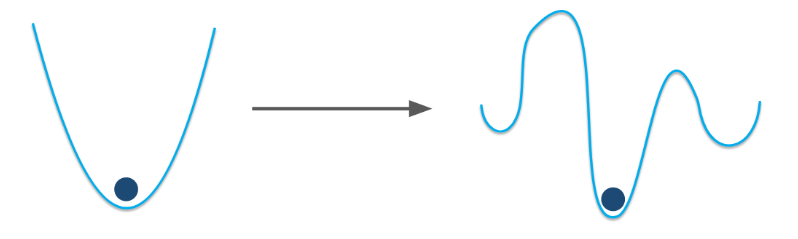
\includegraphics[width=1\textwidth]{figures/algorithme-adiabatique-quantique.png}
        \caption{}
        \label{fig:algorithme-adiabatique-quantique-1}
    \end{subfigure}
    \begin{subfigure}{.48\textwidth}
        \centering
        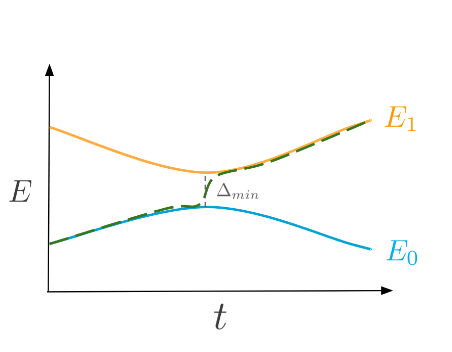
\includegraphics[width=1\textwidth]{figures/algorithme-adiabatique-quantique-2.png}
        \caption{}
        \label{fig:algorithmne-adiabatique-quantique-2}
    \end{subfigure}
    \caption{\textcolor{mydarkred}{\textit{Refaire les figures.}}}
    \label{fig:algorithme-adiabatique-quantique}
\end{figure}

Typiquement, le gap spectral est non-nul~\cite{farhiQuantumComputationAdiabatic2000}, mais cela n'est pas suffisant pour rendre l'algorithme utile comme ce gap doit être assez grand pour limiter le temps d'évolution. Le gap spectral peut être suffisamment grand pour permettre une évolution adiabatique dans un temps réaliste pour certains problèmes, mais ce n'est pas toujours possible~\cite{altshulerAndersonLocalizationMakes2010}. Une alternative consiste à trouver un compromis entre le temps d'évolution et la proximité de l'état final avec l'état fondamental espéré. Le choix du chemin adiabatique utilisé pour transitionner de $H_{D}$ à $H_{P}$ peut aussi différer de l'équation~\ref{eq:chemin-adiabatique} pour maximiser le gap au long du chemin et donc minimiser le temps d'évolution~\cite{nishimoriExponentialEnhancementEfficiency2017, hormoziNonstoquasticHamiltoniansQuantum2017}.

L'algorithme adiabatique quantique se place au sein du \textit{calcul adiabatique quantique}, qui regroupe différentes méthodes similaires. Un autre membre de ce groupe est le \textit{recuit quantique} qui représente généralement l'emploi de QAA dans un environnement bruité, menant ainsi à une version plus réaliste sans contrainte d'adiabaticité ou d'universalité. Cet algorithme partage plusieurs similitudes avec l'algorithme quantique d'optimisation approximative qui seront explorées dans les prochaines sections. 

\textcolor{mydarkred}{\textit{https://arthurpesah.me/assets/pdf/introduction-quantum-annealing.pdf}}

%-----------------------------------------------------------------------------%

\section{Algorithme quantique d'optimisation approximative}

\begin{comment}
\subsection*{Plan}
    
\begin{enumerate}
    \item Expliquer l'histoire et le lien avec le recuit quantique
\end{enumerate}

\subsection*{Références}

1. Farhi, E., Goldstone, J. and Gutmann, S. A Quantum Approximate Optimization Algorithm. Preprint at https://doi.org/10.48550/arXiv.1411.4028 (2014).

2. Kadowaki, T. and Nishimori, H. Quantum annealing in the transverse Ising model. Phys. Rev. E 58, 5355–5363 (1998).

3. Finnila, A. B., Gomez, M. A., Sebenik, C., Stenson, C. and Doll, J. D. Quantum annealing: A new method for minimizing multidimensional functions. Chemical Physics Letters 219, 343–348 (1994).

4. Farhi, E. et al. A Quantum Adiabatic Evolution Algorithm Applied to Random Instances of an NP-Complete Problem. Science 292, 472–475 (2001).

5. Farhi, E., Goldstone, J., Gutmann, S. and Sipser, M. Quantum Computation by Adiabatic Evolution. Preprint at https://doi.org/10.48550/arXiv.quant-ph/0001106 (2000).

6. Parler la adiabatic quantum computation https://arxiv.org/abs/1611.04471
\end{comment}

Bien que le calcul adiabatique quantique soit utilisé pour résoudre les problèmes d'optimisation combinatoire (\textcolor{mydarkred}{\textit{Source?}}), le temps nécessaire pour une évolution adiabatique constitue un facteur limitant pour de nombreux problèmes. L'\textit{algorithme quantique d'optimisation approximative} (« Quantum Approximate Optimization Algorithm ») (QAOA)~\cite{farhiQuantumApproximateOptimization2014} propose ainsi une alternative, un raccourci à l'adiabaticité: la contre-diabacité. \textcolor{mydarkred}{\textit{NOT TRUE I THINK}}

QAOA trouve des bonnes approximations pour de nombreux problèmes d'optimisation, comme les problèmes de coupe maximum
\textcolor{mydarkred}{\textit{Applications}}

De nombreuses extensions à QAOA ont été présentés au cours des dernières années~\cite{blekosReviewQuantumApproximate2024}.

%-----------------------------------------------------------------------------

\subsection{Description de l'algorithme}
\label{subsec:description-algorithme}

\begin{comment}
subsection*{Plan}
    
\begin{enumerate}
    \item Décrire le \textit{Quantum Approximate Optimization Algorithm}
    \item QAOA sees the whole graph?
    \item avantage vs les algorithmes classiques?
\end{enumerate}

\subsection*{Références}

1. Farhi, E., Goldstone, J. and Gutmann, S. A Quantum Approximate Optimization Algorithm. Preprint at https://doi.org/10.48550/arXiv.1411.4028 (2014).
\end{comment}

Étant une idée prometteuse pour les applications des ordinateurs quantiques, l'algorithme quantique d'optimisation approximative a mené à une quantité incroyable de travaux dans les précédentes années. Ainsi, pour simplifier la compréhension de ce concept, l'algorithme original, dû à Farhi, Goldstone et Gutmann~\cite{farhiQuantumApproximateOptimization2014}, est d'abord présenté.

QAOA repose sur deux différents hamiltoniens: l'hamiltonien de problème, ou de phase, $H_{P}$ et l'hamiltonien de forçage, ou de mélange, $H_{D}$. L'hamiltonien de problème est formulé de façon à encoder la solution, potentiellement dégénérée, du problème d'optimisation combinatoire dans son état fondamental. Celui-ci prend typiquement la forme de l'hamiltonien du modèle d'Ising. L'hamiltonien de forçage, quant à lui, est donné par

\begin{equation}
    \label{eq:x-drive}
    H_{D}^{X} = \sum_{i=1}^{n} X_{i} \,,
\end{equation}

où $X_{i}$ est l'opérateur de Pauli $X$ appliqué sur le qubit $i$ d'un système à $n$ qubits. $H_{D}^{X}$ est construit de manière à induire de l'interférence et ainsi permettre l'exploration de l'espace de Hilbert. 

Par définition, l'hamiltonien $H_{p}$ est diagonal dans la base computationnelle, alors que l'hamiltonien $H_{D}$ comprend des termes hors diagonaux de sorte que ceux-ci ne commutent pas entre eux. Deux opérations unitaires paramétrées sont définies à partir des hamiltoniens $H_{P}$ et $H_{D}$: l'opérateur de problème $U_{P}(\gamma) = e^{-i \gamma H_{P}}$ ainsi que l'opérateur de forçage $U_{D}(\beta) = e^{-i \beta H_{D}}$. L'opérateur $U_{P}$ représente une rotation de phase, paramétrisée par $\gamma$, des états de la base computationnelle en fonction de leur énergie donné par $H_{P}$. L'opérateur $U_{D}$, paramétrisé par $\beta$, superpose différents états de la base computationnelle ayant précédemment acquis différents facteurs de phase, menant ainsi à de l'interférence.

En tant que VQA, QAOA est un algorithme hybride composé d'un circuit quantique paramétré et d'un optimiseur classique. Le circuit quantique est d'abord préparé dans un état propre de l'hamiltonien de forçage. Pour l'hamiltonien~\ref{eq:x-drive}, un exemple d'état initial possible est $\ket{\psi_{0}} = \ket{+}^{\otimes n}$. Le produit des opérateurs $U_{D}U_{P}$ est alors appliqué en alternance $p$ fois sur l'état initial $\ket{\psi_{0}}$, donnant l'état suivant:

\begin{equation}
    \label{eq:final-state}
    \ket{\psi(\vec{\gamma}, \vec{\beta})} = \underbrace{U_D(\beta_p) U_P(\gamma_p) \cdots U_D(\beta_1) U_P(\gamma_1)}_{p \text{ fois }} \ket{\psi_{0}} \,,
\end{equation}

où $\vec{\gamma} = (\gamma_{1}, \dots, \gamma_{p})$ et $\vec{\beta} = (\beta_{1}, \dots, \beta_{p})$ sont les paramètres initiaux du circuit. Une fois l'état $\ket{\psi(\vec{\gamma}, \vec{\beta})}$ préparé, la valeur moyenne de l'hamiltonien de problème $H_{P}$ est calculé par des mesures répétées de l'état final dans la base computationnelle:

\begin{equation}
    E_{P} (\vec{\gamma}, \vec{\beta}) = \braket{ \psi(\vec{\gamma}, \vec{\beta}) | H_{P} | \psi(\vec{\gamma}, \vec{\beta}) } \,.
\end{equation}

L'énergie trouvée quantifie l'optimalité de l'état préparé. Par la suite, une méthode d'optimisation classique continue, comme la descente de gradient stochastique, est employé pour mettre à jour itérativement les paramètres $\gamma$ et $\beta$ du circuit paramétré de manière à minimiser la valeur moyenne $E_{P} (\vec{\gamma}, \vec{\beta})$:

\begin{equation}
    (\vec{\gamma}^{*}, \vec{\beta}^{*}) = \arg \min_{{\vec{\gamma}, \vec{\beta}}} E_{P}(\vec{\gamma}, \vec{\beta}) \,.
\end{equation}

Si l'optimisation aboutit de manière espérée, l'état final $\ket{\psi(\vec{\gamma}^{*}, \vec{\beta}^{*})}$ correspond à une superposition des états fondamentaux de $H_{P}$ et donc aux différentes solutions du problème étudié. Si ce n'est pas le cas, le ratio d'approximation $\alpha$ est utilisé pour décrire la qualité de la solution trouvée comme à la section~\ref{sec:intractabilite-approximation-et-optimisation}:

\begin{equation}
    \alpha = \frac{ E_{p} (\vec{\gamma}^{*}, \vec{\beta}^{*})}{\min_{(\vec{\gamma}, \vec{\beta})} E_{p} (\vec{\gamma}, \vec{\beta}) }
\end{equation}

Ce ratio augmente théoriquement avec le nombre de couches $p$ utilisées comme QAOA équivaut à une évolution adiabatique dans la limite $p \to \infty$~\cite{farhiQuantumApproximateOptimization2014}. Notons que pour l'utilisation de QAOA sur des graphes, la valeur de $p$ doit augmenter avec la taille du graphe pour ne pas être limité par la localité de QAOA~\cite{farhiQuantumApproximateOptimization2020}.

L'algorithme se résume par les étapes suivantes, illustrées dans la figure~\ref{fig:qaoa}:

\begin{enumerate}[(1)]
    \item Définition de l'hamiltonien de problème $H_{P}$.
    \item Préparation de l'état initial $\ket{\psi_{0}}$.
    \item Construction du circuit quantique paramétré $\ket{\psi(\gamma, \beta)}$ en appliquant en alternance les opérateurs $U_{P}(\gamma)$ et $U_{D}(\beta)$ $p$ fois.
    \item Calcul de l'énergie $E_{P}$ à travers de mesures dans la base computationnelle.
    \item Optimisation des paramètres $\vec{\gamma}$ et $\vec{\beta}$ à l'aide d'un optimiseur classique minimisant l'énergie $E_{P}$.
\end{enumerate}


\begin{figure}[ht!]
    \centering
    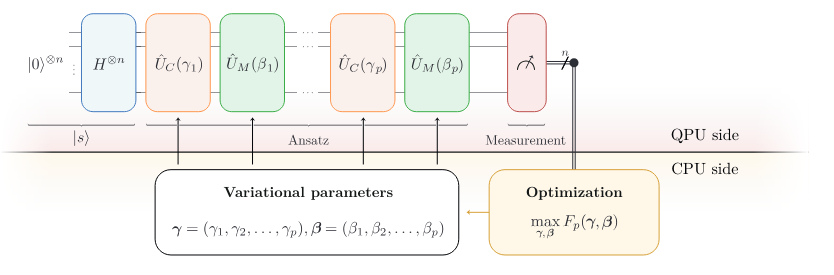
\includegraphics[width=0.7\textwidth]{figures/qaoa.png}
    \caption[Algorithme quantique d'optimisation approximative]{\textcolor{mydarkred}{\textit{Refaire la figure.}}}
    \label{fig:qaoa}
\end{figure}

Décrivons maintenant plus en détails les mécanismes derrière QAOA: la préparation de l'état initial, l'encodage du problème dans un hamiltonien de problème ainsi que le choix de l'hamiltonien de forçage. L'initialisation et l'optimisation des paramètres du circuit est décrit à la section~\ref{subsec:configuration-des-parametres}.

%-----------------------------------------------------------------------------%

\subsubsection{Préparation de l'état initial}
\label{subsec:preparation-de-etat-initial}

Comme QAA, le circuit quantique est initialement préparé dans l'état fondamental de l'hamiltonien de forçage pour garantir le théorème adiabatique. Cependant, la divergence de QAOA du calcul adiabatique implique qu'un autre choix d'état initial peut être choisi. Une alternative consiste à utiliser une solution approximative du problème comme état initial~\cite{eggerWarmstartingQuantumOptimization2021}. 

%-----------------------------------------------------------------------------%

\subsubsection{Encodage du problème}
\label{subsec:encodage-probleme}

\begin{comment}
\subsection*{Plan}

\begin{enumerate}
    \item Introduire la fonction de coût
    \item Introduire le modèle d'Ising et le modèle QUBO
    \item Décrire la transformation d'Ising pour NAE3SAT et 1in3SAT
    \item Prouver la transformation d'Ising pour NAE3SAT et 1in3SAT
\end{enumerate}

\subsection*{Références}

1. Lucas, A. Ising formulations of many NP problems. Frontiers in Physics 2, (2014).
2. MAPPING NP-HARD AND NP-COMPLETE OPTIMISATION PROBLEMS
TO QUADRATIC UNCONSTRAINED BINARY OPTIMISATION PROBLEMS. (CORRECTION DE 1)

\end{comment}

Comment est-ce qu'un problème d'optimisation combinatoire $\varphi(x)$ peut être encodé par un hamiltonien $H_{P}$? D'abord, les entrées $x$ du problème sont caractérisées par une fonction de coût $C(x)$, composés termes de pénalisant les configurations non-valides. Une entrée optimale est associée à un coût nul, alors qu'une entrée non optimale est associée à un coût positif selon sa proximité avec les solutions. Résoudre le problème correspond alors à trouver l'entrée optimale, c'est-à-dire l'entrée $x^{*}$ minimisant la fonction de coût. L'hamiltonien de problème se définit par

\begin{equation}
    H_{P} \ket{x} = C(x) \ket{x}
\end{equation}

Cette équation implique que l'état fondamental de l'hamiltonien $H_{P}$ encode les solutions au problème donné. Un état préparé dans l'état fondamental de $H_{P}$ correspond ainsi à une superposition des solutions au problème $\varphi$. Le modèle d'Ising est fréquemment utilisé pour fournir un hamiltonien décrivant la fonction de coût $C$:

\begin{equation}
    \label{eq:hamiltonien-ising}
    H_P = - \sum_{(i,j) \in E} J_{ij} \sigma_i \sigma_j - \sum_{i \in V} h_i \sigma_i \,,
\end{equation}

où $E$ est l'ensemble d'arêtes, $V$ est l'ensemble de sommets et $\sigma_{i}$ est le spin de la particule $i$. Les constantes $J$ et $h$ représentent respectivement l'interaction entre deux sites et le champ magnétique externe. Le problème d'optimisation quadratique binaire non contraint (« Quadratic Unconstrained Binary Optimization ») (QUBO) permet aussi d'exprimer les fonctions de coût de manière plus générale, en ne les restreignant pas au modèle d'Ising.

\begin{figure}[h]
    \centering
    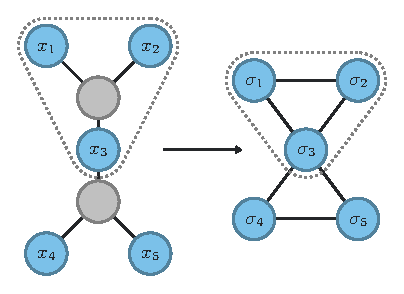
\includegraphics[width=0.55\textwidth]{figures/ising-mapping}
    \caption[Transformation du problème \#NAE3SAT et \#1-in-3SAT au modèle d'Ising]{Exemple de la transformation entre le modèle d'Ising pour NAE3SAT et 1-in-3SAT pour une formule $\varphi$. À gauche, le graphe de facteurs de $\varphi$ avec les sommets de variables (bleus) et de clauses (gris). À droite, le modèle d'Ising correspondant à $\varphi$. Pour 1-in-3SAT, un terme de champ magnétique est ajouté pour favoriser les configurations où chaque clause contienne exactement un variable fixée à 1.}
    \label{fig:transformation-ising}
\end{figure}

Comme trouver l'état fondamental d'un modèle d'Ising constitue un problème \textsf{NP}-complet, il existe alors nécessairement une réduction entre ce problème et les différents problèmes \textsf{NP}-complet. Bien que ces réductions ne sont pas nécessairement évidentes, plusieurs de celles-ci ont été formulées pour le calcul adiabatique quantique~\cite{lucasIsingFormulationsMany2014,lodewijksMappingNPhardNPcomplete2020}. Une réduction intéressante dans notre cas relie le problème positif NAE3SAT au modèle d'Ising antiferromagnétique. Une formule CNF $\varphi$ peut être représentée graphiquement sous la forme d'un graphe bipartie nommé \textit{facteur de graphes}. Dans ce graphe, les clauses et les variables sont représentés sous la forme de sommet alors la présence des variables dans une clause sont représentées à l'aide d'arêtes entre les deux partitions. Considérons pour le moment une seule clause $C = (x_{1} \lor x_{2} \lor x_{3})$ de $\varphi$. En associant chaque variable $x_{i}$ à un spin $\sigma_{i}$ selon la transformation $\sigma_{i} = 1 - 2x_{i}$, cette clause se réduit à un modèle d'Ising en considérant un réseau triangulaire composé des spins $\sigma_{i}$, où chacun de ceux-ci sont reliés aux deux autres spins tels qu'illustré à la figure~\ref{fig:transformation-ising}. L'hamiltonien d'un tel modèle est donné par

\begin{equation}
    H_{P, C} = \sigma_{1}\sigma_{2} + \sigma_{2}\sigma_{3} + \sigma_{3}\sigma_{1}
\end{equation}

Les énergies associées à chaque combinaison possible des spins sont présentés dans le tableau~\ref{tab:energie-nae3sat}, où les spins vers le haut sont représentés par 0 et les spins vers le bas sont représentés par 1. La frustration des spins sur le réseau implique que les seuls états qui ne sont pas dans l'état fondamental sont les états $000$ et $111$. Hors, il s'agit des deux combinaisons ne faisant pas partie de l'ensemble des solutions du problème positif NAE3SAT. L'état fondamental de l'hamiltonien $H_{P, C}$ correspond ainsi bien aux solutions de la clause $C$.

\begin{table*}[h]
    \centering
    \begin{subtable}{0.4\textwidth}
        \centering
        \begin{tabular}{c c}
            \hline
            Entrée & Énergie \\
            \hline
            000 & 3 \\
            001 & -1 \\
            010 & -1 \\
            100 & -1 \\
            011 & -1 \\
            110 & -1 \\
            101 & -1 \\
            111 & 3 \\
            \hline
        \end{tabular}
        \caption{}
        \label{tab:energie-nae3sat}
    \end{subtable}
    % \hspace*{4em}
    \begin{subtable}{0.4\textwidth}
        \centering
        \begin{tabular}{c c}
            \hline
            Entrée & Énergie \\
            \hline
            000 & 0 \\
            001 & -2 \\
            010 & -2 \\
            100 & -2 \\
            011 & 0 \\
            110 & 0 \\
            101 & 0 \\
            111 & 6 \\
            \hline
        \end{tabular}
        \caption{}
        \label{tab:energie-1in3sat}
    \end{subtable}
    \caption{Énergie de chaque entrée dans le modèle d'Ising pour le problème NAE3SAT (a) et 1-in-3SAT (b).}
\end{table*}

La formule est représentable par un modèle d'Ising en appliquant la transformation précédente sur chacune des clauses de la formule, tel qu'illustré à la figure~\ref{fig:transformation-ising}, donnant ainsi l'hamiltonien 

\begin{equation}
    H_{P} = \sum_{C} H_{P, C} \,,
\end{equation}

de manière que chaque clause soit respectée. Ainsi, l'hamiltonien de problème pour NAE3SAT est donné par l'équation~\ref{eq:hamiltonien-ising} avec $J_{ij}=-1$ et $h_{i}=0$. Le problème 1-in-3SAT se transforme au modèle d'Ising en ajoutant pour chaque clause l'hamiltonien

\begin{align*}
   H_{P, C} = \sigma_{1}\sigma_{2} + \sigma_{2}\sigma_{3} + \sigma_{3}\sigma_{1} - \sigma_{1} - \sigma_{2} - \sigma_{3}
\end{align*}

Un champ magnétique externe est ajouté pour imposer la contrainte supplémentaire, c'est-à-dire que toutes les clauses doivent contenir exactement une variable évaluant à vrai. Le tableau~\ref{tab:energie-1in3sat} présente les énergies des configurations pour l'hamiltonien précédent. L'hamiltonien pour le problème 1-in-3SAT est donc donnée par l'équation~\ref{eq:hamiltonien-ising} avec $J_{ij}=-1$ et $h_{i}=1$.

%-----------------------------------------------------------------------------%

\subsubsection{Choix du forçage}

\begin{comment}
\subsection*{Plan}

\begin{enumerate}
    \item Expliquer le but du forçage
    \item Expliquer forçage en X
    \item Expliquer le forçage de Grover
    \item Énumérer les forçages populaires
    \item Est-ce que le mixer doit être un vecteur propre de l'état initial?
\end{enumerate}

\subsection*{Références}
\end{comment}

L'hamiltonien de forçage $H_{D}$ initialement proposé avec QAOA prends son inspiration de l'algorithme adiabatique quantique, en utilisant l'hamiltonien facile à préparer $H_{D}^{X}$. Cela implique que toute la dépendance au problème doit être encodée dans l'hamiltonien de problème $H_{P}$. Comme QAOA n'est pas restreint par cette condition, des opportunités se présentent pour encoder différemment le problème. Par exemple, l'Hamiltonien de forçage peut être utilisé pour restreindre l'espace de Hilbert en prenant en compte la structure du problème. Divers hamiltoniens offrent différentes performances selon le problème étudié. Le choix de forçage demeure encore une question ouverte. 

%-----------------------------------------------------------------------------%

\subsection{Contre-diabacité}

\begin{comment}
    \begin{itemize}
        \item Contre-diabacité
        \item Trottérisation
    \end{itemize}
\end{comment}

Pour établir un lien entre QAA et QAOA, l'évolution de l'hamiltonien doit être rendu discrète. Pour ce faire, la décomposition de Susuki-Trotter au premier ordre, donnée par $e^{A+B} = \lim_{n \to \infty} e^{\frac{A}{n}} e^{\frac{B}{n}}$ pour deux opérateurs $A$ et $B$, est utilisée. Cette décomposition permet de discrétiser l'opérateur d'un hamiltonien $H$ tel que

\begin{equation}
    e^{-i\Delta t H(t)} \approx e^{-i \beta H_D} e^{-i \gamma H_P} + O(\Delta t^2)
\end{equation}

~\cite{wurtzCounterdiabaticityQuantumApproximate2022}

\textcolor{mydarkred}{\textit{Voir mon rapport de stage.}}

\textcolor{mydarkred}{\textit{Expliquer la contre-diabacité.}}

\textcolor{mydarkred}{\textit{Expliquer la trotterisation (voir citation dans notre papier).}}

\textcolor{mydarkred}{\textit{Parler de QAOA lorsque $p \to \infty$}}

\textcolor{mydarkred}{\textit{Level crossings?}}

%-----------------------------------------------------------------------------%

\section{Ansatz quantique à opérateurs alternants}

\begin{comment}
\subsection*{Plan}

\begin{enumerate}
    \item Décrire le \textit{Quantum Alternating Operator Ansatz}
    \item Décrire \textit{Grover-Mixer Quantum Alternating Operator Ansatz}
\end{enumerate}

\subsection*{Références}

1. Hadfield, S. et al. From the Quantum Approximate Optimization Algorithm to a Quantum Alternating Operator Ansatz. Algorithms 12, 34 (2019).

2. Bärtschi, A. and Eidenbenz, S. Grover Mixers for QAOA: Shifting Complexity from Mixer Design to State Preparation. in 2020 IEEE International Conference on Quantum Computing and Engineering (QCE) 72–82 (2020). doi:10.1109/QCE49297.2020.00020.
\end{comment}

L'algorithme quantique d'optimisation approximative applique en alternance un hamiltonien de problème et un hamiltonien de forçage, guidé par l'approche quantique adiabatique. Cet algorithme comporte une limitation importante: les opérateurs appliqués doivent être sous la forme d'une évolution temporelle d'un hamiltonien local fixe. Cette restriction entrave la construction d'opérateurs unitaires potentiellement plus efficaces.

L'\textit{approche quantique des opérateurs alternants} (« Quantum Alternating Operator Ansatz») (QAOA), introduit par Hadfield et coll.~\cite{hadfieldQuantumApproximateOptimization2019}, généralise l'algorithme quantique d'optimisation approximative en permettant l'alternance de familles générales d'opérateurs unitaires paramétrisés plutôt qu'uniquement des opérateurs basés sur un hamiltonien. Cette approche supporte ainsi la représentation d'un plus grand nombre d'états, pouvant possiblement être construit de manière plus efficace. L'algorithme quantique d'approximation quantique et l'approche quantique des opérateurs alternants possèdent le même acronyme. Comme cette dernière étend le premier, l'acronyme QAOA fera référence à l'approche quantique des opérateurs alternant pour le reste de la présente section.

Cette extension trouve son utilité principale dans la création d'opérateurs de forçage. Restreindre l'espace des configurations d'un problème selon les contraintes de celui-ci permet d'éviter une recherche de l'espace de Hilbert complet.


%-----------------------------------------------------------------------------%

\subsection{Description de l'approche}

%-----------------------------------------------------------------------------%




\subsection{Forçage de Grover}

\textit{L'approche quantique des opérateurs alternants avec forçage de Grover} («Grover-Mixer Quantum Alternating Operator Ansatz») (GM-QAOA) fut proposé par Bärtschi et coll.~\cite{bartschiGroverMixersQAOA2020} pour déplacer la complexité de la conception de l'opérateur de forçage à la préparation de l'état initial en s'inspirant de l'algorithme de Grover. 



\begin{equation}
    U_D^{\mathrm{Grover}} = U_{S}\left[ \mathds{1} -\left(1-e^{-i \beta}\right) (\ket{0}\!\bra{0})^{\otimes n} \right] U_{S}^{\dagger} \,,
\end{equation}

\textcolor{mydarkred}{\textit{Décrire l'algorithme de Grover.}}

\begin{figure}[ht!]
    \centering
    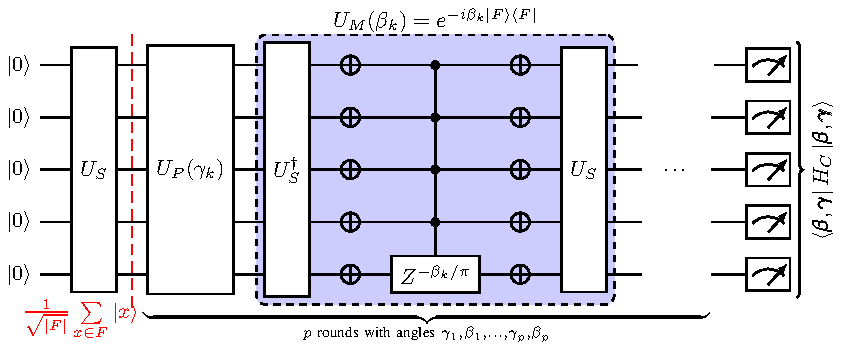
\includegraphics[width=0.8\textwidth]{figures/gm-qaoa}
    \caption[Circuit GM-QAOA]{\textcolor{mydarkred}{\textit{Refaire la figure.}}}
    \label{fig:gm-qaoa}
\end{figure}

%-----------------------------------------------------------------------------%

\section{Configuration des paramètres}
\label{subsec:configuration-des-parametres}

\begin{comment}
\subsection*{Plan}

\begin{enumerate}
    \item Décrire l'importance d'une bonne initialisation des paramètres (\textit{barren plateau}, non-convexité des paramètres)
    \item Énumérer les principales méthodes
    \item Expliquer l'initialisation aléatoire par grille
    \item Expliquer \textit{TQA}
\end{enumerate}

\subsection*{Références}

1. Bittel, L. and Kliesch, M. Training Variational Quantum Algorithms Is NP-Hard. Phys. Rev. Lett. 127, 120502 (2021).

2. Anschuetz, E. R. and Kiani, B. T. Beyond Barren Plateaus: Quantum Variational Algorithms Are Swamped With Traps. Nat Commun 13, 7760 (2022).

3. Akshay, V., Philathong, H., Morales, M. E. S. and Biamonte, J. D. Reachability Deficits in Quantum Approximate Optimization. Phys. Rev. Lett. 124, 090504 (2020).
    
4. Cain, M., Farhi, E., Gutmann, S., Ranard, D. and Tang, E. The QAOA gets stuck starting from a good classical string. Preprint at https://doi.org/10.48550/arXiv.2207.05089 (2022).

Peut-être une référence de plus qui traite directement des barrens plateau?
\end{comment}

La capacité d'entraînement des réseaux de neurones à partir d'une simple descente de gradient fut en partie à l'origine de leur succès retentissant sur de nombreux différents problèmes. L'optimisation des paramètres se fait simplement, même avec des fonctions de coût non convexe, tout en offrant de puissants résultats. Une des attentes des VQA fut de posséder ce même comportement et de pouvoir ainsi pousser les limites des algorithmes variationnels. En effet, l'optimisation classique des paramètres de QAOA fait partie intégrante du concept d'algorithme variationnel quantique. Grâce à celle-ci, il est en théorie possible de prendre avantage des algorithmes quantiques en recourant à des ordinateurs quantiques bruités. Cependant, de nombreuses embûches rendent présentement cette tâche difficile. 

D'abord, l'estimation du gradient de coût est difficile dans de nombreuses situations en raison de la présence de plateaux stériles~\cite{mccleanBarrenPlateausQuantum2018, laroccaReviewBarrenPlateaus2024}, où le gradient devient exponentiellement petit selon la taille du système. Un nombre exponentiel de mesures devient alors nécessaires pour pouvoir identifier la direction minimisant la fonction de coût. Ces complications se présentent surtout pour des circuits de grande profondeur, mais d'autres surgissent même pour ceux de petites tailles. Un grand nombre de minima locaux sont effectivement considérés comme pauvre, c'est-à-dire qu'ils possèdent une énergie petite par rapport au minimum global, augmentant la difficulté d'atteindre une solution approximative de bonne qualité~\cite{anschuetzQuantumVariationalAlgorithms2022}. De plus, l'optimisation des paramètres des VQA est \textsf{NP}-difficile, et donc intraitables dans le pire des cas~\cite{bittelTrainingVariationalQuantum2021}. Ces difficultés sont d'autant plus importantes comme la complexité de l'espace des paramètres augmente avec le nombre de paramètres d'un circuit, impliquant une plus grande difficulté d'optimisation pour les circuits profonds. 

Cet ensemble de complication implique alors qu'une bonne initialisation des paramètres est nécessaire au succès de QAOA. Des paramètres initiaux suffisamment près de l'extremum global peuvent contourner les problèmes énoncés précédemment. L'initialisation de bons paramètres demeure une question ouverte, mais plusieurs approches permettent d'amoindrir ces problèmes. Sack et Serbyn propose entre autres une stratégie d'initialisation basée sur le recuit quantique trottérisé (« Trotterized Quantum Annealing ») (TQA)~\cite{sackQuantumAnnealingInitialization2021}. Cette méthode, utilisé pour les simulations de ce travail,   



%-----------------------------------------------------------------------------%

\section{Échantillonage et biais}
\label{sec:echantillonage-et-biais}

\begin{comment} 
\subsection*{Plan}

\begin{enumerate}
    \item Expliquer l'importance de l'échantillonnage non-biaisé
    \item Expliquer le problème d'échantillonage associé au recuit quantique
    \item Expliquer le problème d'échantillonage associé à QAOA
    \item Expliquer pourquoi GM-QAOA résout ce problème (ne pas oublier d'expliquer les inconvénients de cette méthode)
\end{enumerate}

\subsection*{Références}

1. Zhang, Z. et al. Grover-QAOA for 3-SAT: Quadratic Speedup, Fair-Sampling, and Parameter Clustering. Preprint at https://doi.org/10.48550/arXiv.2402.02585 (2024).

2. Mandrà, S., Zhu, Z. and Katzgraber, H. G. Exponentially Biased Ground-State Sampling of Quantum Annealing Machines with Transverse-Field Driving Hamiltonians. Phys. Rev. Lett. 118, 070502 (2017).

3. Matsuda, Y., Nishimori, H. and Katzgraber, H. G. Ground-state statistics from annealing algorithms: quantum versus classical approaches. New J. Phys. 11, 073021 (2009).

Plus de sources sur le fair sampling pour QAOA?
\end{comment}

L'allure de la distribution obtenue par QAOA est dans notre cas essentiel. Afin de se conformer à la condition de l'algorithme de JVV, celle-ci doit être quasi uniforme comme sans ce critère l'algorithme de JVV n'offre aucune assurance.

Le recuit quantique n'échantillonne pas les états fondamentaux uniformément en général~\cite{matsudaGroundstateStatisticsAnnealing2009, mandraExponentiallyBiasedGroundState2017}. Certains états sont exponentiellement supprimés et nécessitent alors un nombre exponentiel de mesures pour être détectés. Comme le recuit quantique et QAOA sont fortement liés, il est ainsi peu probable que QAOA puisse échantillonner les états fondamentaux de manière uniforme.

Une propriété de l'algorithme GM-QAOA devient alors d'un intérêt considérable: l'équiprobabilité des états de même énergie. Dans GM-QAOA, les solutions sont encodées dans l'état fondamental de l'hamiltonien de problème, ceux-ci posséderont alors la même amplitude et donc la même probabilité. Ainsi, en ne considérant que les solutions, l'état préparé par le circuit GM-QAOA possède toujours une non-uniformité nulle. 
